
\chapter{\propDetTitle}

In Lecture~\ref{elementarydeterminantsII} we \hyperref[detinvertible]{showed} that the determinant of a matrix is non-zero if and only if that matrix is invertible.  We also \hyperref[detmultiplicative]{showed} that the determinant is a \emph{multiplicative} function\index{Multiplicative function}, in the sense that $\det (MN)=\det M \det N$.  Now we will devise some methods for calculating the determinant.

Recall that:
\[
\det M = \sum_{\sigma} \text{sgn}(\sigma) m^1_{\sigma(1)}m^2_{\sigma(2)}\cdots m^n_{\sigma(n)}.
\]

A \emph{minor}\index{Minor} of an $n\times n$ matrix $M$ is the determinant of any square matrix obtained from $M$ by deleting one row and one column.  In particular, any entry $m^i_j$ of a square matrix~$M$ is associated to a minor obtained by deleting the $i$th row and $j$th column of~$M$.

It is possible to write the determinant of a matrix in terms of  its minors\index{Expansion by minors} as follows:

\begin{eqnarray*}
\det M &=& \sum_{\sigma} \text{sgn}(\sigma)\, m^1_{\sigma(1)}m^2_{\sigma(2)}\cdots m^n_{\sigma(n)} \\
&=& m^1_1\, \sum_{\hat{\sigma}} \text{sgn}(\hat{\sigma})\, m^2_{\hat{\sigma}(2)}\cdots m^n_{\hat{\sigma}(n)} \\
& -&  m^1_2\, \sum_{\hat{\sigma}} \text{sgn}(\hat{\sigma})\, m^2_{\hat{\sigma}(1)}m^3_{\hat{\sigma}(3)}\cdots m^n_{\hat{\sigma}(n)} \\
& +&  m^1_3\,  \sum_{\hat{\sigma}} \text{sgn}(\hat{\sigma})\, m^2_{\hat{\sigma}(1)}m^3_{\hat{\sigma}(2)}m^4_{\hat{\sigma}(4)}\cdots m^n_{\hat{\sigma}(n)} \pm \cdots
\end{eqnarray*}
Here the symbols $\hat{\sigma}$ refer to permutations of $n-1$ objects.  What we're doing here is collecting up all of the terms of the original sum that contain the first row entry $m^1_j$ for each column number $j$.  Each term in that collection is associated to a permutation sending $1\rightarrow j$.  The remainder of any such permutation maps the set $\{2, \ldots, n \}\rightarrow \{1, \ldots, j-1, j+1, \ldots, n \}$.  We call this partial permutation $\hat{\sigma}=\begin{bmatrix} \sigma(2) & \cdots & \sigma(n) \end{bmatrix}$.

The last issue is that the permutation $\hat{\sigma}$ may not have the same sign as $\sigma$.  From previous homework, we know that a permutation has the same parity as its inversion number.  Removing $1\rightarrow j$ from a permutation  reduces the inversion number by the number of elements right of $j$ that are less than~$j$.  Since $j$ comes first in the permutation $\begin{bmatrix}j & \sigma(2) & \cdots & \sigma(n) \end{bmatrix}$, the inversion number of $\hat{\sigma}$ is reduced by $j-1$.  Then the sign of~$\sigma$ differs from the sign of~$\hat{\sigma}$ if $\sigma$ sends $1$ to an even number.

In other words, to expand by minors we pick an entry $m^1_j$ of the first row, then add $(-1)^{j-1}$ times the determinant of the matrix with row $i$ and column~$j$ deleted.

\begin{example}
Let's compute the determinant of 
$M=\begin{pmatrix}
1 & 2 & 3 \\
4 & 5 & 6 \\
7 & 8 & 9 \\
\end{pmatrix}$ using expansion by minors.

\begin{eqnarray*}
\det M & = & 1\det \begin{pmatrix}
5 & 6 \\
8 & 9 \\
\end{pmatrix}
-2 \det \begin{pmatrix}
4 & 6 \\
7 & 9 \\
\end{pmatrix}
+3 \det \begin{pmatrix}
4 & 5 \\
7 & 8 \\
\end{pmatrix} \\
& = & 1(5\cdot 9- 8\cdot 6) -2 (4\cdot 9- 7\cdot 6) + 3 (4\cdot 8- 7\cdot 5) \\
& = & 0 \\
\end{eqnarray*}
Here, $M^{-1}$ does not exist because\footnote{A fun exercise is to compute the determinant of a $4\times 4$ matrix filled in order, from left to right,  with the numbers $1,2,3,\ldots 16$. What do you observe? Try the same for a $5\times 5$ matrix with $1,2,3\ldots 25$. Is there a pattern? Can you explain it?} $\det M=0.$
\end{example}


\begin{example}
Sometimes the entries of a matrix allow us to simplify the calculation of the determinant.  Take $N= \begin{pmatrix}
1 & 2 & 3 \\
4 & 0 & 0 \\
7 & 8 & 9 \\
\end{pmatrix}$.  Notice that the second row has many zeros; then we can switch the first and second rows of $N$ to get:

\begin{eqnarray*}
\det \begin{pmatrix}
1 & 2 & 3 \\
4 & 0 & 0 \\
7 & 8 & 9 \\
\end{pmatrix} & = & -\det \begin{pmatrix}
4 & 0 & 0 \\
1 & 2 & 3 \\
7 & 8 & 9 \\
\end{pmatrix}\\
&=& -4 \det \begin{pmatrix}
2 & 3 \\
8 & 9 \\
\end{pmatrix} \\
&=& 24
\end{eqnarray*}
\end{example}
 
\videoscriptlink{properties_of_determinant_practice.mp4}{Example}{video_properties_of_determinant_practice}

\begin{theorem}
For any square matrix $M$, we have:
\[
\det M^T = \det M
\]
\end{theorem}
\begin{proof}
  By definition, \[
\det M = \sum_{\sigma} \text{sgn}(\sigma) m^1_{\sigma(1)}m^2_{\sigma(2)}\cdots m^n_{\sigma(n)}.
\]

For any permutation $\sigma$, there is a unique inverse permutation $\sigma^{-1}$ that undoes $\sigma$.  If $\sigma$ sends $i\rightarrow j$, then $\sigma^{-1}$ sends $j\rightarrow i$.  In the two-line notation for a permutation, this corresponds to just flipping the permutation over.  For example, if $\sigma=\begin{bmatrix} 
1 & 2 & 3 \\
2 & 3 & 1
\end{bmatrix}$, then we can find $\sigma^{-1}$ by flipping the permutation and then putting the columns in order:

\[
\sigma^{-1}=\begin{bmatrix} 
2 & 3 & 1 \\
1 & 2 & 3
\end{bmatrix}=\begin{bmatrix} 
1 & 2 & 3 \\
3 & 1 & 2
\end{bmatrix}
\]
Since any permutation can be built up by transpositions, one can also find the inverse of a permutation $\sigma$ by undoing each of the transpositions used to build up $\sigma$; this shows that one can use the same number of transpositions to build $\sigma$ and $\sigma^{-1}$.  In particular, $\sgn \sigma= \sgn \sigma^{-1}$.

%\begin{center}\href{\webworkurl ReadingHomework14/1/}{Reading homework: problem 14.1}\end{center}
\reading{14}{1}

Then we can write out the above in formulas as follows:
\begin{eqnarray*}
\det M &=& \sum_{\sigma} \text{sgn}(\sigma) m^1_{\sigma(1)}m^2_{\sigma(2)}\cdots m^n_{\sigma(n)} \\
&=& \sum_{\sigma} \text{sgn}(\sigma) m_1^{\sigma^{-1}(1)}m_2^{\sigma^{-1}(2)}\cdots m_n^{\sigma^{-1}(n)} \\
&=& \sum_{\sigma} \text{sgn}(\sigma^{-1}) m_1^{\sigma^{-1}(1)}m_2^{\sigma^{-1}(2)}\cdots m_n^{\sigma^{-1}(n)} \\
&=& \sum_{\sigma} \text{sgn}(\sigma) m_1^{\sigma(1)}m_2^{\sigma(2)}\cdots m_n^{\sigma(n)} \\
&=& \det M^T.
\end{eqnarray*}
The second-to-last equality is due to the existence of a unique inverse permutation: summing over permutations is the same as summing over all inverses of permutations.  The final equality is by the definition of the transpose.
\end{proof}

\begin{center}

\includegraphics[scale=.25]{\propDetPath/detMT.jpg}
\end{center}

\begin{example}
Because of this theorem, we see that expansion by minors also works over columns.  Let $M=\begin{pmatrix}
1 & 2 & 3 \\
0 & 5 & 6 \\
0 & 8 & 9 \\
\end{pmatrix}$.  Then $$\det M = \det M^T = 1\det \begin{pmatrix}
5 & 8 \\
6 & 9 \\
\end{pmatrix}=-3\, .$$
\end{example}

\section{Determinant of the Inverse}

Let $M$ and $N$ be $n\times n$ matrices.
We previously showed that 

\[
\det (MN)=\det M \det N \text{, and } \det I=1.
\]
Then $1 = \det I = \det (MM^{-1}) = \det M \det M^{-1}$.  As such we have:
\begin{theorem}
\[
\det M^{-1} = \frac{1}{\det M}
\]
\end{theorem}

Just so you don't forget this:
\begin{center}

\includegraphics[scale=.3]{\propDetPath/detMm1.jpg}
\end{center}


\section{Adjoint of a Matrix}


Recall that for the $2\times 2$ matrix 
%\begin{figure}
\begin{center}
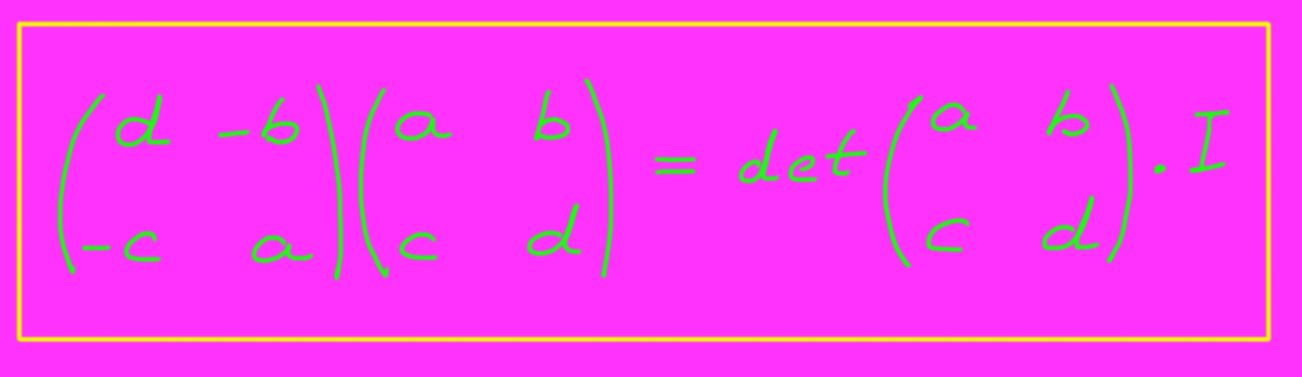
\includegraphics[scale=.2]{\propDetPath/adj2x2.jpg}
\end{center}
%\end{figure}
Or in a more careful notation: if
$M=\begin{pmatrix}
m^1_1 & m^1_2 \\
m^2_1 & m^2_2 \\
\end{pmatrix}$, then $$M^{-1}=\frac{1}{m^1_1m^2_2-m^1_2m^2_1}\begin{pmatrix}
m^2_2 & -m^1_2 \\
-m^2_1 & m^1_1 \\
\end{pmatrix}\, ,$$
so long as $\det M=m^1_1m^2_2-m^1_2m^2_1\neq 0$.
  The  matrix $\begin{pmatrix}
m^2_2 & -m^1_2 \\
-m^2_1 & m^1_1 \\
\end{pmatrix}$ that appears above is a special matrix, called the \emph{adjoint} of $M$.  Let's define the adjoint for an $n \times n$ matrix.


The \emph{cofactor}\index{Cofactor} of $M$ corresponding to the entry $m^i_j$ of $M$ 
%and then deleting the $i$th row and $j$th column of $M$, taking the determinant of the 
is the prooduct of the minor associated to $m^i_j$
%resulting matrix, and 
%multiplying by
times $(-1)^{i+j}$.  This is written $\cofactor(m^i_j)$.

\begin{definition}
For $M=(m^i_j)$ a square matrix, The \emph{adjoint matrix} $\adj M$ is given by:
\[
\adj M = (\cofactor(m^i_j))^T
\]
\end{definition}

\begin{example}
\[
\adj \begin{pmatrix}
3 & -1 & -1 \\
1 & 2 & 0 \\
0 & 1 & 1 \\
\end{pmatrix}
=
\begin{pmatrix}
\det \begin{pmatrix}
2 & 0 \\
1 & 1 
\end{pmatrix}
& -\det \begin{pmatrix}
1 & 0 \\
0 & 1 
\end{pmatrix}
& \det \begin{pmatrix}
1 & 2 \\
0 & 1 
\end{pmatrix}
\\
-\det \begin{pmatrix}
-1 & -1 \\
1 & 1 
\end{pmatrix}
& \det \begin{pmatrix}
3 & -1 \\
0 & 1 
\end{pmatrix}
& -\det \begin{pmatrix}
3 & -1 \\
0 & 1 
\end{pmatrix}
\\
\det \begin{pmatrix}
-1 & -1 \\
2 & 0 
\end{pmatrix}
& -\det \begin{pmatrix}
3 & -1 \\
1 & 0 
\end{pmatrix}
& \det \begin{pmatrix}
3 & -1 \\
1 & 2 
\end{pmatrix}
\\
\end{pmatrix}^T
\]
\end{example}

%\begin{center}\href{\webworkurl ReadingHomework14/2/}{Reading homework: problem 14.2}\end{center}
\reading{14}{2}

Let's multiply $M\adj M$.  For any matrix $N$, the $i, j$ entry of $MN$ is given by taking the dot product of the $i$th row of $M$ and the $j$th column of $N$.  
Notice that the dot product of the $i$th row of $M$ and the $i$th column of $\adj M$ is just the expansion by minors of $\det M$ in the $i$th row.
Further, notice that the dot product of the $i$th row of $M$ and the $j$th column of $\adj M$ with $j\neq i$ is the same as expanding $M$ by minors, but with the $j$th row replaced by the $i$th row.  Since the determinant of any matrix with a row repeated is zero, then these dot products are zero as well.

We know that the $i,j$ entry of the product of two matrices is the dot product of the $i$th row of the first by the $j$th column of the second.  Then:
\[
M\adj M = (\det M) I
\]

Thus, when $\det M\neq 0$, the adjoint gives an explicit formula for $M^{-1}$.


\begin{theorem}
For $M$ a square matrix with $\det M\neq 0$ (equivalently, if $M$ is invertible), then
\[
M^{-1}=\frac{1}{\det M}\adj M
\]
\end{theorem}

\videoscriptlink{properties_of_determinant_adjoint.mp4}{The Adjoint Matrix}{video_properties_of_determinant_adjoint}


\begin{figure}
\begin{center}

\includegraphics[scale=.3]{\propDetPath/adjM.jpg}
\end{center}
\end{figure}

\begin{example}
Continuing with the previous example,
\[
\adj \begin{pmatrix}
3 & -1 & -1 \\
1 & 2 & 0 \\
0 & 1 & 1 \\
\end{pmatrix} = \begin{pmatrix}
2 & 0 & 2 \\
-1 & 3 & -1 \\
1 & -3 & 7 \\
\end{pmatrix}.
\]

Now, multiply:

\begin{eqnarray*}
\begin{pmatrix}
3 & -1 & -1 \\
1 & 2 & 0 \\
0 & 1 & 1 \\
\end{pmatrix}
\begin{pmatrix}
2 & 0 & 2 \\
-1 & 3 & -1 \\
1 & -3 & 7 \\
\end{pmatrix}
&=&
\begin{pmatrix}
6 & 0 & 0 \\
0 & 6 & 0 \\
0 & 0 & 6 \\
\end{pmatrix} \\[1mm]
\Rightarrow \begin{pmatrix}
3 & -1 & -1 \\
1 & 2 & 0 \\
0 & 1 & 1 \\
\end{pmatrix}^{-1} & = & \frac{1}{6}\begin{pmatrix}
2 & 0 & 2 \\
-1 & 3 & -1 \\
1 & -3 & 7 \\
\end{pmatrix}
\end{eqnarray*}

This process for finding the inverse matrix is sometimes called \emph{Cramer's~Rule}~\index{Cramer's rule}.
\end{example}

\section{Application: Volume of a Parallelepiped}

Given three vectors $u,v,w$ in $\Re^3$, the parallelepiped\index{Parallelepiped} determined by the three vectors is the ``squished'' box whose edges are parallel to $u, v$, and $w$ as depicted in Figure~\ref{parallelepiped}.

From calculus, we know that the volume of this object is $|u\dotprod (v\times w)|$.  This is the same as expansion by minors of the matrix whose columns are $u,v,w$.  Then:
\[
\text{Volume}=\big|\det \begin{pmatrix}u & v & w \end{pmatrix} \big|
\] 



\begin{figure}
\begin{center}
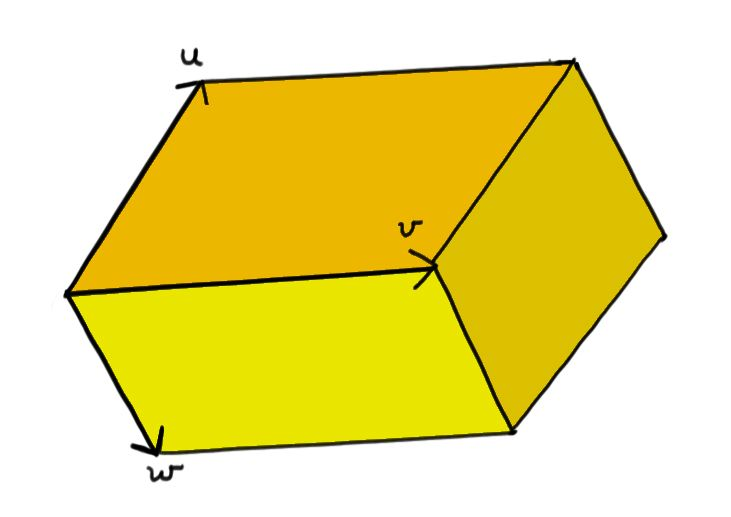
\includegraphics[scale=.4]{parallelepiped.jpg}
\caption{A parallelepiped.\label{parallelepiped}}
\end{center}
\end{figure}



%\section*{References}
%Hefferon, Chapter Four, Section I.1 and I.3
%\\
%Beezer, Chapter D, Section DM, Subsection DD
%\\
%Beezer, Chapter D, Section DM, Subsection CD
%\\
%Wikipedia:
%\begin{itemize}
%\item \href{http://en.wikipedia.org/wiki/Determinant}{Determinant}
%\item \href{http://en.wikipedia.org/wiki/Elementary_matrix}{Elementary Matrix}
%\item \href{http://en.wikipedia.org/wiki/Cramers_rule}{Cramer's Rule}
%\end{itemize}




\section{Review Problems}



\begin{enumerate}

\item While performing  Gaussian elimination on these augmented matrices write the full system of equations describing the new rows in terms of the old rows above each equivalence symbol as in  \hyperlink{Keeping track of EROs with equations between rows}{Example}~\ref{Rsystem}. 
$$
\begin{amatrix}{2} 
2 & 2 & 10 \\
1 & 2 & 8 \\
\end{amatrix}
,~
\begin{amatrix}{3} 
1 & 1 & 0 & 5 \\
1 & 1 & \!\!-1& 11 \\
-1 & 1 & 1 & -5 \\ 
\end{amatrix}
$$

%%%%%%%%%%%%%%%%%%%

\item Solve the vector equation by applying ERO matrices to each side of the equation to perform elimination. Show each matrix explicitly as in \hyperlink{Undoing}{Example~\ref{slowly}}.

\begin{eqnarray*}
\begin{pmatrix}
3	&6 	&2 \\ %-3
5 	&9 	&4 \\ %1
2	&4	&2 \\ %0
\end{pmatrix} 
\begin{pmatrix}
 x \\ 
y \\
z 
\end{pmatrix} 
=
\begin{pmatrix}
-3 \\ 
1  \\
0  \\
\end{pmatrix} 
\end{eqnarray*}

%%%%%%%%%%%%%%%%%%%

\item Solve this vector equation by finding the inverse of the matrix through $(M|I)\sim (I|M^{-1})$ and then applying $M^{-1}$ to both sides of the equation. 
\begin{eqnarray*}
\begin{pmatrix}
2	&1 	&1 \\ %9
1 	&1 	&1 \\ %6
1	&1	&2 \\ %7
\end{pmatrix} 
\begin{pmatrix}
 x \\ 
y \\
z 
\end{pmatrix} 
=
\begin{pmatrix}
9 \\ 
6  \\
7  \\
\end{pmatrix} 
\end{eqnarray*}


%%%%%%%%%%%%%%%%%%%

\item Follow the method of  \hyperlink{elldeeeww}{Examples~\ref{factorize} and~\ref{factorizes}} to find the $LU$ and $LDU$ factorization of 
\begin{eqnarray*}
\begin{pmatrix}
3	&3 	&6 \\ %0 %2
3 	&5 	&2 \\ %1 %1
6	&2	&5 \\ %0 %1
\end{pmatrix} .
\end{eqnarray*}



%%%%%%%%%%%%%%%%%%%%

\item 
Multiple matrix equations with the same matrix can be solved simultaneously. 
\begin{enumerate}
\item Solve both systems by performing elimination on just one augmented matrix.
\begin{eqnarray*}
\begin{pmatrix}
2	&-1 	&-1 \\ %0 %2
-1 	&1 	&1 \\ %1 %1
1	&-1	&0 \\ %0 %1
\end{pmatrix} 
\begin{pmatrix}
 x \\ 
y \\
z 
\end{pmatrix} 
=
\begin{pmatrix}
0\\ 
1  \\
0  \\
\end{pmatrix} 
,~
\begin{pmatrix}
2	&-1 	&-1 \\ %0 %2
-1 	&1 	&1 \\ %1 %1
1	&-1	&0 \\ %0 %1
\end{pmatrix} 
\begin{pmatrix}
 a \\ 
b \\
c 
\end{pmatrix} 
=
\begin{pmatrix}
2\\ 
1  \\
1  \\
\end{pmatrix} 
\end{eqnarray*}
\item Give an interpretation of the columns of $M^{-1}$ in $(M|I)\sim (I|M^{-1})$ in terms of solutions to certain systems of linear equations.
\end{enumerate}

%%%%%%%%%%%%%%%%%%%%%%%%

\item How can you convince your fellow students to never make this mistake?
\begin{eqnarray*}
\begin{amatrix}{3} 
1 & 0 & 2 & 3 \\ 
0 & 1 & 2& 3 \\
2 & 0 & 1 & 4 \\
\end{amatrix} 
& 
\stackrel{R_1'=R_1+R_2}{
\stackrel{R_2'=R_1-R_2}{ 
\stackrel{\ R_3'= R_1+2R_2}{\sim}}}
&
\begin{amatrix}{3} 
1 & 1 & 4 & 6 \\
1 & \!\!-1 & 0& 0 \\
1 & 2 & 6 & 9 
\end{amatrix}
\end{eqnarray*}

\item Is $LU$ factorization of a matrix unique?  Justify your answer.


\item[$\infty$.] If you randomly create a matrix by picking numbers out of the blue, it will probably be difficult to perform elimination or factorization; fractions and large numbers will probably be involved. To invent simple problems it is better to start with a simple answer:
\begin{enumerate}
\item Start with any augmented matrix in RREF. Perform EROs to make most of the components non-zero. Write the result on a separate piece of paper and give it to your friend. Ask that friend to find RREF of the augmented matrix you gave them. Make sure they get the same augmented matrix you started with.  
\item Create  an upper triangular matrix $U$ and a lower triangular matrix~$L$ with only $1$s on the diagonal. Give the result to a friend to factor into $LU$ form. 
\item Do the same with an $LDU$ factorization. 
\end{enumerate}
\end{enumerate}

\phantomnewpage



\newpage




